\documentclass[journal]{IEEEtran}

% Math
\usepackage{amsmath,amssymb,amsfonts,amsthm,mathtools}

% Typography and figures
\usepackage[utf8]{inputenc}
\usepackage[T1]{fontenc}
\usepackage{hyperref}
\usepackage{url}
\usepackage{booktabs}
\usepackage{nicefrac}
\usepackage{microtype}
\usepackage{xcolor}
\usepackage{graphicx}
\usepackage{subcaption}
\usepackage{multirow}
\usepackage{array}
\usepackage{tabularx}
\usepackage{makecell}
\usepackage{algorithm}
\usepackage{algpseudocode}
\usepackage{cite}
\usepackage{tikz}
\usetikzlibrary{arrows.meta,positioning,shapes.geometric,fit,calc}
\usepackage{fontawesome5}

% cleveref must be loaded AFTER hyperref
\usepackage[capitalize,noabbrev]{cleveref}

% Theorems
\theoremstyle{plain}
\newtheorem{theorem}{Theorem}
\newtheorem{proposition}[theorem]{Proposition}
\newtheorem{lemma}[theorem]{Lemma}
\newtheorem{corollary}[theorem]{Corollary}
\theoremstyle{definition}
\newtheorem{definition}[theorem]{Definition}
\newtheorem{assumption}[theorem]{Assumption}
\theoremstyle{remark}
\newtheorem{remark}[theorem]{Remark}
\crefname{assumption}{Assumption}{Assumptions}
\Crefname{assumption}{Assumption}{Assumptions}

% math_commands.tex -- shared notation for FLAS
% Graph / network model
\newcommand{\setG}{\mathcal{G}}
\newcommand{\setV}{\mathcal{V}}
\newcommand{\setE}{\mathcal{E}}
\newcommand{\setF}{\mathcal{F}}
\newcommand{\Cv}{C_v}
\newcommand{\Mv}{M_v}

% Cryptographic objects
\newcommand{\skey}{K}
\newcommand{\domid}{\mathsf{d}}
\newcommand{\fl}{\mathsf{FL}}
\newcommand{\mtag}{\tau}
\newcommand{\seq}{\mathsf{seq}}

% Operators
\DeclareMathOperator{\prf}{PRF}
\DeclareMathOperator{\mac}{MAC}
\DeclareMathOperator{\Verify}{Verify}
\DeclareMathOperator{\Encode}{Encode}


\title{6FLAS: A Lightweight Security Protection Mechanism for LEO Satellite Networks Using IPv6 Flow Label and SRv6}

\author{Anonymous Authors%
\thanks{Evaluation scripts, prototype benchmarks, and generated data are publicly available at \url{https://github.com/nongfude/6Flas}.}%
}

\begin{document}
\maketitle

\begin{abstract}
Low Earth orbit (LEO) satellite constellations are becoming a backbone of 6G
non-terrestrial networks, yet their open inter-satellite links (ISLs) are
exposed to eavesdropping, injection, and replay, while on-board routers offer
too little compute and memory to run conventional per-flow security such as
IPsec or DTLS. This paper presents 6FLAS, a lightweight, stateless security protection
mechanism that moves security state off the satellite and into the packet
itself. 6FLAS repurposes the 20-bit IPv6 Flow Label as a connectionless flow
authenticator and binds it to an SRv6 security segment, so each on-board router
verifies a single keyed message authentication code (MAC) over the routing
header using only a small per-direction replay window rather than a per-flow
security association table. The LEO security problem is formalized on a
resource-constrained directed graph; the 6FLAS packet format, per-hop
verification algorithm, and a security argument against eavesdropping,
forgery, man-in-the-middle, replay, and stateless-denial-of-service attacks are
provided. 6FLAS is evaluated with a reproducible analytical processing model, an
event-driven latency model of a 1584-satellite Walker-delta constellation,
and a Python software prototype that validates the structural ordering on
commodity hardware.
Analytically projected on a 1\,GHz space-grade core, 6FLAS reduces per-hop
security processing time by about $48\times$ versus IPsec ESP and $5.9\times$
versus an SRv6 HMAC baseline; the Python prototype confirms the structural
ordering on commodity hardware ($3.6\times$ over an SRv6-Sec baseline). 6FLAS
cuts per-packet byte overhead by $79\%$ and eliminates per-flow on-board state
entirely (zero bytes per flow versus $256$\,B for IPsec~ESP), while keeping the
end-to-end latency within propagation-dominated bounds. These results indicate
that packet-carried, topology-aware security is a practical fit for the
resource envelope of LEO on-board routers.

\end{abstract}

\begin{IEEEkeywords}
LEO satellite networks, IPv6 Flow Label, SRv6, lightweight authentication, network security, non-terrestrial networks.
\end{IEEEkeywords}

\section{Introduction}
\label{sec:intro}

\IEEEPARstart{L}{ow} Earth orbit (LEO) satellite constellations have moved from
proposal to deployment: mega-constellations now place thousands of satellites
at altitudes of a few hundred kilometers, and standards bodies position them as
a backbone of 6G non-terrestrial networks (NTN), delivering low-latency global
connectivity where terrestrial infrastructure is absent~\cite{mahboob,kodheli2021,3gppntn}. Unlike bent-pipe relays, modern constellations forward
traffic in space over inter-satellite links (ISLs), so a packet may traverse
many on-board IP routers before reaching a ground gateway~\cite{handley,bhattacherjee2022}.

This in-orbit forwarding is exactly what makes security hard. ISLs are
broadcast over open free-space channels, and the published, near-deterministic
orbital geometry lets an adversary with a suitable terminal predict when and
where a link will exist, then eavesdrop, inject, or replay
traffic~\cite{yue,wu2024leosec,du2025leosec,tang2026satdef,giuliari}. At the same time, an on-board
router runs on a radiation-hardened processor with a fraction of the compute
and memory of a terrestrial core router, and it cannot be patched or rebooted
on demand~\cite{denby}. The result is a sharp mismatch: the threat
surface grows with every added hop, while the per-hop security budget is tiny.


Conventional IP security was designed for endpoints with ample resources and
stable associations. IPsec ESP and DTLS protect a flow by maintaining a
per-flow security association (SA) holding keys, selectors, counters, and a
replay window, and by encrypting and authenticating every packet with
heavyweight primitives~\cite{rfc4301,rfc6347}. This model assumes endpoints
with sufficient memory and relatively stable associations; on a constellation
carrying $10^5$--$10^6$ concurrent flows, the aggregate SA state and per-packet
crypto exceed the on-board budget, and the frequent ISL handovers caused by
orbital motion force costly SA re-establishment, with measurement and modeling
studies of satellite IPsec reporting significant handover and renegotiation
costs~\cite{yue}.

Protocols closer to the space and routing layers help but do not close the gap.
At the link layer, the CCSDS Space Data Link Security protocol authenticates and
encrypts a single space link~\cite{ccsds}; it is effective hop-by-hop but
provides neither end-to-end protection across an in-orbit IP path nor any use of
the network-layer routing information that LEO IP forwarding already carries.
Segment Routing over IPv6 (SRv6) brings programmable source routing to the
satellite data plane and is attractive for LEO because a ground controller can
pin a path through a predictable
constellation~\cite{rfc8402,rfc8754,rfc8986,rfc9252}; the SRH defines an HMAC TLV to
authenticate the segment list and recent work proposes richer security
SIDs~\cite{rfc8754,srsurvey,abdelsalam2021}, but the HMAC TLV authenticates the whole segment
list with a full SHA-256 digest that is expensive to verify on every hop, and
existing SRv6 security designs still assume per-flow or per-policy state at
verifying nodes~\cite{abdelsalam2021,tanveer2024srv6sec}.

Lightweight cryptography supplies fast building blocks but not the missing
systems design. A large body of work, including the NIST
lightweight-cryptography standardization and software-friendly keyed PRFs such
as SipHash, offers primitives suited to constrained
hardware~\cite{nistlwc,simon,siphash,lv2025leolwc}, yet these do not by themselves answer
where to keep security state or how to verify packets at line rate on an
on-board router. Finally, the 20-bit IPv6 Flow Label is set by the source,
immutable in transit, and today used only for ECMP load balancing and QoS
classification~\cite{rfc6437,rfc6438}; to our knowledge it has not been
developed as a network-layer security authenticator with a defined derivation
and verification rule, leaving its potential as a security primitive
unexploited.


The key insight is that security state should reside in the packet rather than
on the satellite, while the structured, predictable LEO topology makes per-hop
checks trivial. This insight is realized in \textbf{6FLAS} (IPv6 \textbf{F}low \textbf{L}abel
\textbf{A}uthenticated \textbf{S}egments), a lightweight security mechanism
that (i) repurposes the IPv6 Flow Label as a connectionless flow authenticator
derived from a pre-shared domain key, and (ii) binds it to an SRv6 security
segment so that every on-board router verifies a single short keyed MAC over
the routing header, using only a small per-direction replay window instead of a
per-flow SA table. Because the Flow Label is set by the source and is immutable
in transit by design~\cite{rfc6437}, it is a natural carrier for a stable, source-bound flow-identity token. Because LEO routers forward over a small
number of fixed grid directions, the egress check that normally requires a
routing lookup collapses to a constant-time comparison.


This paper makes four contributions, each addressing a gap above.

\begin{itemize}

\item \textbf{Packet-carried stateless security model for LEO.}
We formalize LEO security on a resource-constrained directed graph and show how
moving security state from on-board storage into the packet meets the
data-origin authentication, integrity, anti-replay, and access-control
requirements without per-flow SAs (\cref{sec:method}).

\item \textbf{Flow-Label-based stateless flow authenticator.}
We define a flow as a five-tuple plus a security-domain identifier, derive the
20-bit Flow Label from a domain key, and give a stateless verification rule that
needs no per-flow table walk (\cref{sec:fl-auth}).

\item \textbf{SRv6 Security SID integration.}
We integrate the authenticator with SRv6 through a Security SID
(Locator$\,|\,$Function$\,|\,$Arguments) that encodes a path security policy and
specializes per-hop checking to the six fixed LEO forwarding directions, while
interoperating with nodes that implement the base \texttt{End} behavior (\cref{sec:srv6-bind}).

\item \textbf{Security argument and reproducible evaluation.}
We analyze resilience to eavesdropping, forgery, man-in-the-middle, replay, and
stateless DoS, and quantify cost with an explicit processing model and an
event-driven latency model of a 1584-satellite constellation
(\cref{sec:security,sec:exp}).

\end{itemize}


On a 1\,GHz space-grade core, 6FLAS verifies a packet in about $306$\,ns per hop,
roughly $48\times$ faster than IPsec ESP and $5.9\times$ faster than an SRv6
HMAC baseline (analytically projected on a 1\,GHz space-grade core); it adds only $8$ bytes per packet ($79\%$ less than IPsec ESP)
and carries zero per-flow on-board state ($100\%$ reduction versus IPsec~ESP; total fixed state is $192$\,B, direction-scoped). Under a $10^6$-flow load its single-core forwarding throughput is about
$48\times$ that of IPsec ESP, and its end-to-end latency stays within the
propagation-dominated regime of the constellation.

The remainder of this paper is organized as follows.
\cref{sec:prelim} gives the LEO,
Flow Label, and SRv6 background, the threat model, and the problem
formulation. \cref{sec:method} presents 6FLAS. \cref{sec:security} analyzes its
security, and \cref{sec:exp} reports the evaluation. \cref{sec:conclusion}
concludes.

\section{IPv6-Enabled LEO Network Model and Problem Formulation}
\label{sec:prelim}

This section establishes the network model and problem formulation. The LEO
constellation is first described as a network of IPv6/SRv6 on-board routers and
the topological regularities that constrain the design space; the
two IPv6 features central to lightweight per-hop security — the Flow Label and
SRv6 — are then reviewed. The adversary and the security and design requirements
are subsequently stated, and the whole problem is finally cast as a feasibility
condition on a resource-constrained graph. \cref{fig:model} previews the model: an IPv6/SRv6
data plane carried in orbit, the open links an adversary can reach, and the
packet fields available for protection.

\begin{figure}[t]
\centering
\resizebox{\columnwidth}{!}{%
\footnotesize
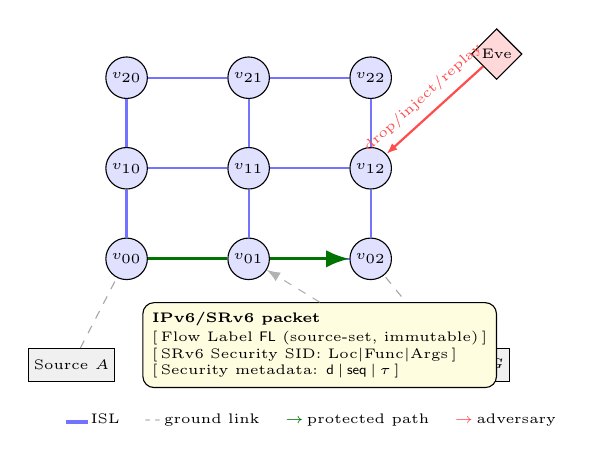
\begin{tikzpicture}[
    sat/.style={circle,draw,fill=blue!12,minimum size=15pt,inner sep=0pt,font=\tiny},
    gnd/.style={rectangle,draw,fill=gray!12,minimum size=12pt,inner sep=2pt,font=\tiny},
    adv/.style={diamond,draw,fill=red!15,minimum size=12pt,inner sep=1pt,font=\tiny},
    isl/.style={-,thick,blue!55},
    gl/.style={-,dashed,gray!70},
    atk/.style={-{Latex[length=4pt]},red!70,thick},
    >=Latex]
% satellite grid (3 planes x 3)
\foreach \r in {0,1,2} {
  \foreach \c in {0,1,2} {
    \node[sat] (s\r\c) at (1.55*\c, 1.15*\r) {$v_{\r\c}$};
  }
}
% intra-plane (horizontal) ISLs
\foreach \r in {0,1,2} { \foreach \c in {0,1} {
  \pgfmathtruncatemacro{\cn}{\c+1}
  \draw[isl] (s\r\c) -- (s\r\cn);
}}
% inter-plane (vertical) ISLs
\foreach \c in {0,1,2} { \foreach \r in {0,1} {
  \pgfmathtruncatemacro{\rn}{\r+1}
  \draw[isl] (s\r\c) -- (s\rn\c);
}}
% ground nodes
\node[gnd] (src) at (-0.7,-1.35) {Source $A$};
\node[gnd] (gw)  at (4.2,-1.35) {Gateway $G$};
\draw[gl] (src) -- (s00);
\draw[gl] (gw)  -- (s02);
% highlight an end-to-end path A -> v00 -> v01 -> v02 -> G
\draw[->,very thick,green!45!black] (s00) -- (s01) -- (s02);
% adversary
\node[adv] (e) at (4.7,2.6) {Eve};
\draw[atk] (e) -- node[pos=0.50,above,sloped,font=\fontsize{5}{6}\selectfont,red!70]{drop/inject/replay} (s12);
% packet field box
\node[draw,rounded corners,fill=yellow!12,font=\tiny,align=left,anchor=north west] (pkt)
  at (0.2,-0.55)
  {\textbf{IPv6/SRv6 packet}\\[1pt]
   $[$\,Flow Label $\fl$ (source-set, immutable)\,$]$\\
   $[$\,SRv6 Security SID: Loc$|$Func$|$Args\,$]$\\
   $[$\,Security metadata: $\domid\,|\,\seq\,|\,\mtag$\,$]$};
\draw[->,dashed,gray!60,thin] (pkt.north) -- (s01);
% legend
\node[font=\tiny,anchor=west] at (-0.9,-2.05)
  {\textcolor{blue!55}{\rule{8pt}{1.2pt}}\,ISL \quad
   \textcolor{gray!70}{-\,-}\,ground link \quad
   \textcolor{green!45!black}{$\rightarrow$}\,protected path \quad
   \textcolor{red!70}{$\rightarrow$}\,adversary};
\end{tikzpicture}%
}
\caption{IPv6-enabled LEO network model. Each satellite is an IPv6/SRv6 on-board
router; intra- and inter-plane ISLs form a regular $+$Grid, and ground links
attach sources and gateways. Because every link is an open free-space channel,
an adversary (Eve) can eavesdrop, inject, or replay on any ISL or ground link
(\cref{sec:threat}).}
\label{fig:model}
\end{figure}

\subsection{LEO Satellite Network Characteristics}
\label{sec:leo-char}

The constellation under consideration is a Walker-delta LEO configuration: $P$ orbital planes each carrying
$S$ satellites at altitude $h$ of a few hundred kilometers (using the
Starlink-like shell $h=550$\,km, $P=72$, $S=22$, $N=PS=1584$ in
\cref{sec:exp}). Each satellite is an on-board IP router connected to its
neighbors by ISLs. In the common $+$Grid pattern, a satellite maintains four
ISLs: two intra-plane links to the satellites ahead and behind, and two
inter-plane links to satellites in adjacent planes; together with the
up/down ground-link direction, this yields a small, fixed set of forwarding
directions per node.

Two properties shape the design space. First, the topology is
\emph{dynamic but predictable}: satellites move continuously, ISLs are made and
broken on handover, yet positions and contact windows follow published
ephemerides and can be computed in advance~\cite{handley,giuliari,kassing2023}. Second,
on-board resources are \emph{severely constrained}: a radiation-hardened
processor offers far less compute, memory, and energy than a terrestrial router,
and software updates are slow and risky~\cite{denby,del2019}. A security
mechanism for LEO must therefore have low per-packet processing cost, low
per-flow memory, and must tolerate frequent topology changes without expensive
re-keying.

\subsection{IPv6 Flow Label and SRv6 Primer}
\label{sec:fl-srv6}

Two features already present in every IPv6/SRv6 packet are central to
lightweight per-hop security: the 20-bit Flow Label, which the source sets and
routers must not modify, and the Segment Routing Header, which lets a controller
express and enforce an explicit forwarding path. The following paragraphs review
each in turn.

\paragraph{IPv6 Flow Label.}
The IPv6 header carries a 20-bit Flow Label field. By RFC~6437~\cite{rfc6437}
the label is set by the source node, should be uniform across a flow's packets,
and \emph{must not be modified by routers in transit}; routers use it as an
opaque key for ECMP and QoS without interpreting its
value~\cite{rfc6438}. The field thus provides up to $2^{20}=1{,}048{,}576$
distinct values that travel unmodified end-to-end. These two properties,
source-set and immutable, are precisely what a stateless flow authenticator
needs.

\paragraph{SRv6.}
Segment Routing over IPv6 expresses an explicit path as an ordered list of
128-bit SIDs carried in the Segment Routing Header (SRH)~\cite{rfc8402,rfc8754,srsurvey}. A SID follows a \texttt{Locator$\,|\,$Function$\,|\,$Arguments}
structure~\cite{rfc8986}: the Locator routes the packet toward the SID's owner,
the Function selects a behavior at that node (e.g., \texttt{End}, \texttt{End.X}
forwarding to a specific link), and the Arguments parameterize it. A node
processing the SRH advances the Segments Left pointer and applies the behavior
of the current SID. SRv6 lets a source or controller program an end-to-end path
through the constellation~\cite{michel2019,bhattacherjee2020}, and the SRH also defines an optional HMAC TLV to
authenticate the segment list~\cite{rfc8754,abdelsalam2021}.

\subsection{Threat Model and Security Requirements}
\label{sec:threat}


A Dolev--Yao--style network adversary adapted to LEO is assumed: the adversary
can (i) \emph{eavesdrop} on any ISL or ground link, since the orbital channel
is open and the geometry is predictable; (ii) \emph{inject} arbitrary packets,
including spoofed source addresses and forged headers; and (iii) \emph{replay}
previously observed packets, possibly from a different vantage point. The
adversary is assumed \emph{unable} to physically tamper with on-board hardware or extract
keys from a satellite's secure element, and cannot break standard cryptographic
primitives. Satellites within a security domain share keys provisioned
out-of-band before launch or via a separate key-management channel; key
management is orthogonal to this work and domain keys are treated as given.


The mechanism must provide: \textbf{(R1) data-origin authentication}, a router
can confirm a packet originates from an authorized source in its domain;
\textbf{(R2) routing-header integrity}, tampering with the protected span
(IPv6 base header $+$ SRH $+$ 8-byte metadata, $72$\,B) is detected —
payload integrity and confidentiality are explicitly out of scope;
\textbf{(R3) anti-replay}, replayed packets are rejected; and \textbf{(R4)
access control}, only packets bound to an authorized path/policy are forwarded.


In addition, the mechanism must have \textbf{(D1)} low per-hop processing
overhead, \textbf{(D2)} low per-flow on-board storage, and \textbf{(D3)}
robustness to LEO topology dynamics (handovers without per-flow re-keying).

\subsection{Problem Formulation}
\label{sec:formulation}

The constellation at a routing epoch is modeled as a directed graph
$\setG=(\setV,\setE)$, where $\setV$ is the set of $N$ on-board routers and
$(u,v)\in\setE$ is an active ISL or ground link. Each node $v\in\setV$ has a
compute budget $\Cv$ (cycles available per packet at line rate) and a memory
budget $\Mv$ (bytes for security state). A flow $f$ is a stream of packets from
an authorized source traversing a path $\pi_f=(v_0,v_1,\dots,v_\ell)$ in
$\setG$. Let $\setF$ be the set of concurrent flows, with $|\setF|$ up to
$10^6$.

A per-hop security mechanism $\mathcal{M}$ is defined by a verification cost
$c_{\mathcal{M}}$ (cycles per packet per hop) and a per-flow state cost
$m_{\mathcal{M}}$ (bytes per flow per node). Feasibility under
\cref{sec:leo-char} requires, for every node $v$ on the busiest path,
\begin{equation}
\label{eq:feasibility}
c_{\mathcal{M}} \le \Cv
\quad\text{and}\quad
\sum_{f:\,v\in\pi_f} m_{\mathcal{M}} \le \Mv .
\end{equation}
The goal is to design $\mathcal{M}$ that satisfies the security requirements
R1--R4 while minimizing $c_{\mathcal{M}}$ and, crucially, the per-flow term
$m_{\mathcal{M}}$, since the state cost in \cref{eq:feasibility} scales with the
number of flows crossing a node. Stateful mechanisms make
$m_{\mathcal{M}}=\Theta(1)$ \emph{per flow} (a full SA), so the left-hand sum
grows linearly in the flow count; the ideal mechanism targets $m_{\mathcal{M}}\to 0$
per flow by carrying the security context in the packet, leaving only a bounded
per-direction replay window at each node, independent of $|\setF|$.

\section{6FLAS: Lightweight Security Mechanism}
\label{sec:method}

This section presents 6FLAS. The two design principles that motivate the
mechanism are introduced first, followed by its two cooperating carriers: a
Flow-Label-based stateless flow authenticator and an SRv6-integrated security
segment that drives constant-time per-hop verification. Domain key management
and an end-to-end walk-through of the data path conclude the section. Throughout, the design keeps a single invariant in view: the only mutable on-board state is a small
per-direction replay window, never anything per flow.
\cref{fig:arch} shows the overall architecture.

\begin{figure}[t]
\centering
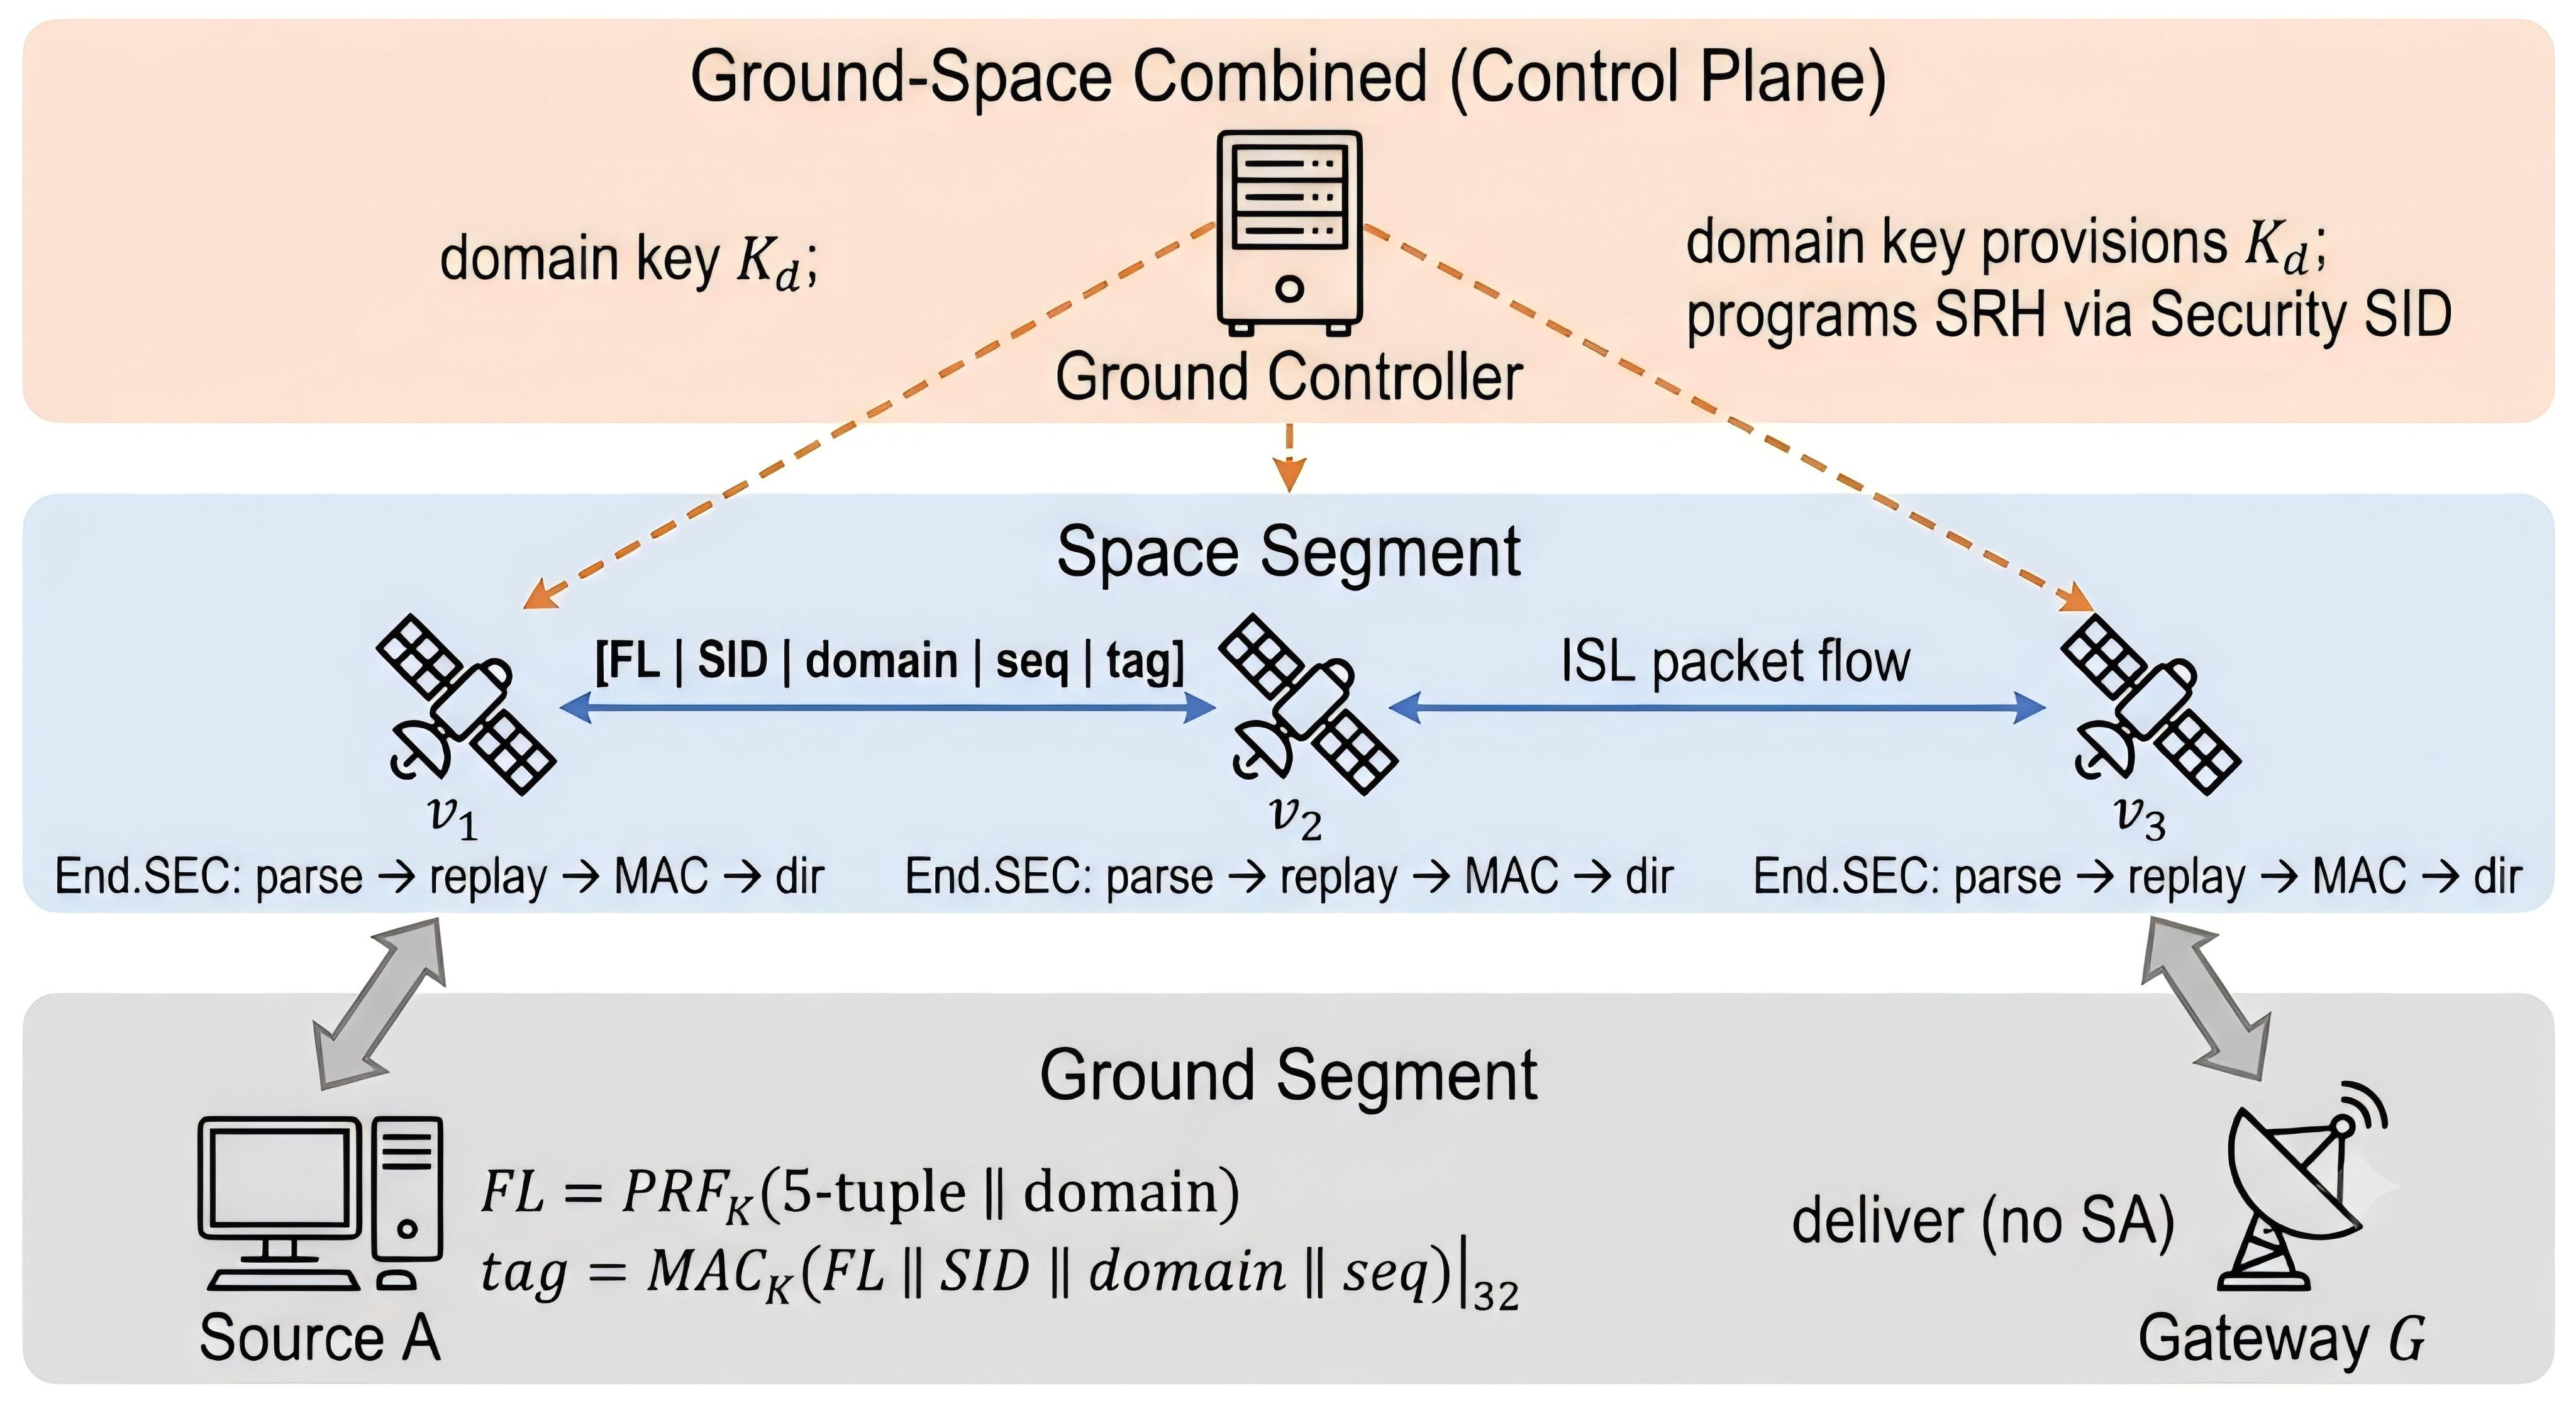
\includegraphics[width=\columnwidth]{figures/arch.jpg}
\caption{6FLAS three-segment architecture.
\textit{Ground segment}: source $A$ computes the Flow Label
$\fl=\prf_{\skey_\domid}(\textit{5-tuple}\,\|\,\domid)$ and the 32-bit MAC tag
before transmission; gateway $G$ delivers packets with no per-flow SA.
\textit{Space segment}: each on-board router executes the four-step
\texttt{End.SEC} procedure (\cref{alg:verify}) over ISLs — no per-flow state
migrates on handover.
\textit{Ground-space combined (control plane)}: the ground controller provisions
domain key $\skey_\domid$ to all nodes and programs the SRH path via Security SIDs;
bidirectional arrows denote space-ground uplinks.}
\label{fig:arch}
\end{figure}

\subsection{Design Philosophy}
\label{sec:philosophy}

6FLAS rests on two ideas. First, \emph{carry security state in the packet, not on
the satellite}. A stateful protocol stores a security association per flow at
every protected node; 6FLAS instead derives a compact authenticator from a
domain key and embeds it in fields the packet already carries, so a verifying
router needs no per-flow record. This drives the per-flow state term
$m_{\mathcal{M}}$ in \cref{eq:feasibility} toward zero and makes the mechanism
indifferent to ISL handovers: when a flow is rerouted, no SA migrates because
none exists. Second, \emph{exploit the structured LEO topology}. Because each
router forwards over a small fixed set of grid directions
(\cref{sec:leo-char}), the egress access-control check, which on a general
router needs a routing/policy lookup, becomes a constant-time comparison
against the SID-encoded expected direction.

The two carriers are complementary. The immutable, source-set Flow Label
(\cref{sec:fl-srv6}) supplies a stable, source-bound flow-identity token that is
the same at every hop; the SRv6 Security SID supplies the per-hop path policy
and the bytes over which integrity is checked. \cref{fig:overview} shows the
resulting packet and the per-hop pipeline.

\begin{figure}[t]
\centering
\footnotesize
\setlength{\fboxsep}{4pt}
\fbox{\parbox{\dimexpr\columnwidth-2\fboxsep-2\fboxrule\relax}{\centering
\textbf{IPv6 base header} \;[\,\textbf{Flow Label} $\fl$ = $\prf_{\skey_\domid}(\text{5-tuple}\,\|\,\domid)$\,] \\[2pt]
$\downarrow$ \\[2pt]
\textbf{SRH} \;[\,Segment list $\;\dots\;$ \textbf{Security SID} = Loc$\,|\,$Func$\,|\,$Args\,] \\[2pt]
$\downarrow$ \\[2pt]
\textbf{6FLAS metadata (8\,B)}: \;[\,domain $\domid$ | seq $\seq$ | tag $\mtag$\,] \\[2pt]
$\downarrow$ \\[2pt]
\textbf{Payload} (optionally encrypted, out of scope)
}}
\caption{6FLAS packet structure. The Flow Label carries a stateless flow
authenticator; the SRv6 Security SID encodes the per-hop path policy; an
8-byte metadata block carries the domain id, sequence number, and truncated MAC
tag. Each on-board router verifies the tag over the covered routing span and
checks the replay window, then forwards.}
\label{fig:overview}
\end{figure}

\subsection{Flow-Label-Based Stream Authentication}
\label{sec:fl-auth}

\begin{definition}[Authenticated flow]
\label{def:flow}
A 6FLAS flow is the tuple $f=(\textsf{5tuple},\domid)$ where \textsf{5tuple} is
the IPv6 five-tuple (source/destination address, source/destination port,
next-header) and $\domid$ is a security-domain identifier shared by the
authorized routers serving the flow.
\end{definition}

The source node sets the Flow Label deterministically from the flow and the
domain key $\skey_\domid$:
\begin{equation}
\label{eq:fl}
\fl \;=\; \prf_{\skey_\domid}(\textsf{5tuple}\,\|\,\domid) \bmod 2^{20},
\end{equation}
where $\prf$ is a keyed pseudorandom function (using a SipHash-class keyed
PRF~\cite{siphash}). By RFC~6437 the label is then immutable in
transit~\cite{rfc6437}, so $\fl$ is a stable, source-bound token that every hop
observes identically. Because $\skey_\domid$ is secret, an off-path adversary
cannot compute the label that a given five-tuple should carry, and an on-path
adversary that copies $\fl$ cannot reuse it for a different five-tuple without
detection (the per-packet MAC below binds them together). The 20-bit space
admits up to $2^{20}\approx 1.05$M concurrent labels per domain; collision
behavior under heavy load is discussed in the evaluation.

Each packet carries an 8-byte 6FLAS metadata block: a 1-byte domain id $\domid$,
a 3-byte monotonically increasing sequence number $\seq$, and a 4-byte
truncated MAC tag
\begin{equation}
\label{eq:tag}
\mtag \;=\; \mac_{\skey_\domid}\!\bigl(\fl \,\|\, \textsf{SID} \,\|\, \domid \,\|\, \seq\bigr)\big|_{32},
\end{equation}
computed over the immutable Flow Label, the active Security SID, the domain id,
and the sequence number. A verifying router recomputes \cref{eq:tag} from
fields already in the packet plus the domain key it holds; no per-flow state is
consulted. The tag binds the flow identity ($\fl$), the path policy
(\textsf{SID}), and the freshness ($\seq$) together, so altering any of them
invalidates the tag (R1, R2). \cref{sec:security} bounds the forgery
probability of the 32-bit truncation.

The 3-byte sequence counter $\seq$ resets on each transport-level reconnection,
and domain-key rotation implicitly invalidates old counters, so rollover is not
a concern in normal operation. The per-direction replay window $W_v$ uses a
$w=256$-entry bitmap (32\,B per direction), giving a total on-board state of
$6\times32=192$\,bytes for the six $+$Grid directions — independent of the flow
count and well within any space-grade processor's memory budget.

\subsection{SRv6 Security Segment and Per-Hop Verification}
\label{sec:srv6-bind}

6FLAS encodes its per-hop policy in an SRv6 Security SID that follows the
standard \texttt{Locator$\,|\,$Function$\,|\,$Arguments} layout~\cite{rfc8986}.
The \texttt{End.SEC} function is defined as a strict superset of \texttt{End},
so nodes that implement only \texttt{End} continue forwarding without
interruption.

\begin{definition}[Security SID behavior \texttt{End.SEC}]
\label{def:endsec}
When a router $v$ receives a packet whose active SID carries the \texttt{End.SEC}
function code, it executes \cref{alg:verify} before performing the standard
SRv6 \texttt{End}/\texttt{End.X} forwarding action. If any check in
\cref{alg:verify} fails, the packet is dropped and no SRv6 processing occurs.
If all checks pass, $v$ advances the Segments Left pointer, applies the standard
SRv6 forwarding action for the next SID, and advances the replay window. A node
that implements \texttt{End} but not \texttt{End.SEC} performs standard
\texttt{End}/\texttt{End.X} forwarding without the security checks, interoperating
with the overlay but providing no per-hop verification.
\end{definition}

\begin{itemize}
    \item \textbf{Locator} (64\,b): routes the packet toward the next 6FLAS node,
    exactly as in standard SRv6.
    \item \textbf{Function} (16\,b): a code point \texttt{End.SEC} that triggers
    6FLAS verification before the usual \texttt{End}/\texttt{End.X} forwarding.
    \item \textbf{Arguments} (48\,b): the path security policy, encoding the
    expected ingress direction, the authorized egress direction (one of the six
    fixed LEO grid directions), and a domain/policy tag matched against $\domid$.
\end{itemize}

Encoding the expected egress direction in the SID is what lets a router enforce
access control (R4) without a routing-table or policy lookup: the controller
that programs the path writes the intended next direction into the SID at
source time, and each hop simply checks that its actual forwarding direction
matches. \cref{tab:args} shows the 48-bit Arguments field layout.

\begin{table}[t]
\centering
\caption{6FLAS Security SID Arguments field (48 bits total).}
\label{tab:args}
\renewcommand{\arraystretch}{1.2}
\begin{tabular}{lrl}
\toprule
\textbf{Field} & \textbf{Bits} & \textbf{Description} \\
\midrule
Ingress dir.   & 4  & Expected ingress dir.\ (3\,b index + 1\,b reserved) \\
Egress dir.    & 4  & Authorized egress dir.\ (3\,b index + 1\,b reserved) \\
Domain id      & 8  & Matches $\domid$ in 6FLAS metadata block \\
Path-policy    & 32 & Controller-set policy hash for the flow group \\
\bottomrule
\end{tabular}
\end{table}

\paragraph{Per-hop verification}
\label{sec:perhop}
\cref{alg:verify} gives the per-hop procedure. After parsing the IPv6 base
header and the active SID, the router (1) hashes the Flow Label into a small
per-direction replay-window table to locate the relevant window in $O(1)$,
(2) checks the sequence number against the sliding window for anti-replay (R3),
(3) recomputes the MAC of \cref{eq:tag} and compares it in constant time to the
carried tag (R1, R2), and (4) checks that the SID-encoded egress direction is
one of the node's authorized directions before forwarding (R4). Every step uses
only fields in the packet and the domain key; there is no per-flow SA lookup.

\begin{algorithm}[t]
\caption{6FLAS per-hop verification at router $v$}
\label{alg:verify}
\begin{algorithmic}[1]
\Require packet $p$; domain keys $\{\skey_\domid\}$; replay windows $W_v[\,\cdot\,]$
\State $(\fl,\textsf{SID},\domid,\seq,\mtag) \gets \textsc{Parse}(p)$
\If{$\domid \notin$ authorized domains at $v$} \State \textbf{drop} \EndIf
\State $w \gets W_v[\,\textsf{hash}(\fl)\ \%\ |W_v|\,]$ \Comment{$O(1)$ window select}
\If{$\seq \le w.\text{base}$ \textbf{or} $w.\text{seen}(\seq)$}
    \State \textbf{drop} \Comment{replayed / stale (R3)}
\EndIf
\State $\mtag' \gets \mac_{\skey_\domid}(\fl \,\|\, \textsf{SID} \,\|\, \domid \,\|\, \seq)\big|_{32}$
\If{$\mtag' \neq \mtag$} \State \textbf{drop} \Comment{forged / tampered (R1,R2)} \EndIf
\State $\text{dir} \gets \textsc{Egress}(\textsf{SID.Args})$
\If{$\text{dir} \notin$ authorized directions at $v$}
    \State \textbf{drop} \Comment{policy violation (R4)}
\EndIf
\State $w.\textsc{Advance}(\seq)$; \quad \textsc{ApplySRv6}(p); \quad \textbf{forward}
\end{algorithmic}
\end{algorithm}

\paragraph{Topology-aware optimization and statelessness.}
A general router enforcing an egress policy would consult a forwarding or
policy table whose size grows with the number of destinations. In a $+$Grid LEO
node the authorized egress set has at most six members (north/south intra-plane,
east/west inter-plane, up/down ground), so line~11 of \cref{alg:verify} is a
comparison against a six-element fixed set, i.e., constant time and constant
space, independent of $|\setF|$. Likewise the replay window table $W_v$ is sized
per direction, not per flow, so its memory is $O(1)$ in the flow count. These
specializations are what make 6FLAS satisfy the feasibility condition
\cref{eq:feasibility} at $10^6$ flows where stateful schemes do not. The only
mutable state a 6FLAS router keeps is the bounded per-direction replay window
$W_v$, independent of the number of flows: many flows hash into the same window,
and the window only tracks recently seen sequence numbers within a time horizon.
Thus $m_{\mathcal{M}}$ per flow is effectively zero, and
a handover that reroutes a flow requires no state transfer, directly satisfying
D2 and D3.

\paragraph{Hardware pipeline mapping.}
\cref{alg:verify} decomposes into four stages with no inter-stage feedback:
(1)~header parse and domain-id gate, (2)~replay-window probe,
(3)~MAC recompute, and (4)~direction check and window advance.
Stages~2 and~4 access only the 192-byte on-chip SRAM described above; stage~3
feeds the keyed-MAC core directly from parsed header fields with no memory
indirection. Because stage~3 is the critical-path stage (${\approx}306$\,ns at
1\,GHz), throughput is limited by the MAC core rather than any data-dependent
memory access, and a pipelined implementation sustains one verification per
MAC-core cycle. This pipeline structure is exactly what makes 6FLAS amenable
to FPGA or ASIC realization on a space-grade logic fabric~\cite{li2022}: the
critical path is a fixed-width keyed-hash, and the only state written back per
packet is a single bit in the 192-byte replay bitmap.

\subsection{Domain Key Management}
\label{sec:keymgmt}

6FLAS verification requires each authorized router to hold the domain key
$\skey_\domid$; a full key-management protocol is out of scope~\cite{tan2025crossdomain},
but the stateless design keeps the overhead light. The domain key is a symmetric
secret shared among all nodes in domain $\domid$; large constellations partition
into multiple domains (up to 256 via the 1-byte $\domid$ field) to bound the
blast radius of a compromise. Each satellite is provisioned at manufacture or via
a secured telecommand channel with the keys of the domains it serves.
Ground terminals acting as packet sources are similarly provisioned through
the same ground-based key-management channel, since computing $\fl$
(\cref{eq:fl}) and the initial tag (\cref{eq:tag}) both require $\skey_\domid$;
the security perimeter of a domain thus spans all authorized senders and
verifiers sharing $\skey_\domid$. Rotation
follows an epoch schedule: the operator pushes $\skey_{\domid}^{(e+1)}$ to all
nodes before epoch $e{+}1$ begins; verifiers accept both the current and the
immediately previous epoch to absorb in-flight packets. Because updates are
domain-granular, bandwidth scales as $O(|D|)$, not $O(|\setF|)$ — for 256
domains with 128-bit keys, each epoch push is only $4096$\,bytes. Revocation
rotates the affected domain key and immediately invalidates any traffic an
adversary could mint; because 6FLAS holds no per-flow secrets, revocation
granularity is the domain, which is coarse but cheap.

To make the data path concrete, consider a packet from source $A$ to gateway $G$
routed through three on-board nodes $v_1{\to}v_2{\to}v_3$ in domain
$\domid{=}7$. At the source, $A$ computes
$\fl=\prf_{\skey_7}(\textsf{5tuple}\,\|\,7)\bmod 2^{20}$, writes it into the
IPv6 Flow Label, pushes an SRH whose active Security SID at each hop encodes the
intended egress direction (e.g., \texttt{east}, \texttt{north}, \texttt{down}),
sets $\seq$ from its per-flow counter, and computes the $32$-bit tag
$\mtag=\mac_{\skey_7}(\fl\,\|\,\textsf{SID}\,\|\,7\,\|\,\seq)|_{32}$. At $v_1$,
the router reads $\domid{=}7$ (authorized), selects the replay window by
$\textsf{hash}(\fl)$, checks $\seq$, recomputes the tag over the same span and
matches it, confirms its egress is \texttt{east}, advances the window, and
forwards. Nodes $v_2$ and $v_3$ repeat the identical $O(1)$ check against their
own authorized directions. No node ever created, looked up, or migrated a
per-flow record; if an ISL break reroutes the flow through a different $v_2'$,
that node verifies the next packet with $\skey_7$ exactly as $v_2$ would have,
with no re-keying.

\section{Security Analysis}
\label{sec:security}

We analyze 6FLAS against the threat model of \cref{sec:threat}. Throughout, let
$\skey_\domid$ be the secret domain key, assume the keyed PRF/MAC is a secure
pseudorandom function, and recall that the Flow Label is immutable in transit.

\subsection{Resilience to Known Attacks}
\label{sec:attacks}

We examine 6FLAS against the four attack classes that follow from the
threat model: forgery and tampering, replay, man-in-the-middle
manipulation, and stateless denial of service. 

\paragraph{Forgery and tampering (R1, R2).}
A packet is accepted only if the carried tag equals
$\mtag=\mac_{\skey_\domid}(\fl\,\|\,\textsf{SID}\,\|\,\domid\,\|\,\seq)|_{32}$
(\cref{eq:tag}, \cref{alg:verify}). An adversary without $\skey_\domid$ who
modifies any covered field, the flow identity $\fl$, the path policy
\textsf{SID}, the domain id, or the sequence number, must produce a matching
tag.

\begin{proposition}[Forgery bound]
\label{prop:forgery}
Against an adversary making $q$ verification queries and lacking $\skey_\domid$,
the probability that any single forged or tampered packet is accepted is at most
$2^{-32}+\epsilon_{\prf}$, where $\epsilon_{\prf}$ is the PRF-distinguishing
advantage for the keyed MAC.
\end{proposition}

The $2^{-32}$ term is the chance of guessing the 32-bit truncated tag; a secure
MAC contributes only $\epsilon_{\prf}$. We prove this in \cref{sec:formal}.
Truncating to 32 bits trades tag length for header
compactness; a wider tag can be used when a stronger bound is required. Because the tag covers \textsf{SID}, an adversary also cannot
redirect a packet onto an unauthorized path without invalidating it (R4).

\paragraph{Replay (R3) — probabilistic guarantee.}
Each accepted packet advances the per-direction sliding window $W_v$
(\cref{alg:verify}, lines 4--6, 12). Because the window is shared among
\emph{all flows in a direction} rather than keyed per flow, R3 carries a
probabilistic qualifier: replay of $(\fl_A, \seq_n)$ is detected while
$\seq_n$ remains within the $w$-entry window, but escapes only if other flows
in the same direction collectively advance the window base past $\seq_n$ within
the timing tolerance $\Delta$.

\begin{proposition}[Replay-window eviction bound]
\label{prop:replay}
Let $k = |F_{d,\domid}|$ be the number of flows sharing direction $d$ and
domain $\domid$ in a single replay-window bucket, and let $R_{d,\domid}$ be
their aggregate packet rate. A replayed $\seq_n$ is guaranteed rejected for
at least $\lfloor w/R_{d,\domid} \rfloor$ seconds after first acceptance
($w=256$); at $R_{d,\domid}=10^4$\,pkt/s this covers $25$\,ms. Beyond that
interval, clock-based rejection (tolerance $\Delta$) applies. The probability
of false-positive rejection from two distinct flows coinciding on the same
current sequence number is $O(k^2/2^{24})$, valid when
$k \ll \sqrt{2^{24}} \approx 4{,}096$. With $256$ domains and $6$ forwarding
directions the worst-case bucket at $10^6$ total flows holds
$\lfloor 10^6/(256{\times}6) \rfloor \approx 651$ flows, well within this bound.
\end{proposition}

At the operating rates of \cref{sec:results}, each per-direction window retains
a sequence number for several milliseconds; with $\Delta$ set to cover
propagation delay, the combined guarantee is sufficient for the LEO threat model.
Clock-based rejection is the primary mechanism for long-lived flows whose
sequence numbers have long since left the sliding window.

\paragraph{Man-in-the-middle.}
An on-path adversary can observe and relay packets but cannot alter the covered
fields without breaking \cref{prop:forgery}, and cannot splice a valid tag from
one flow onto another because the tag binds $\fl$ (the per-flow identity) to the
SID and sequence number. Downgrade to plain SRv6 is detected because a 6FLAS
domain expects the \texttt{End.SEC} function and a valid tag; a packet lacking
them is dropped at the first 6FLAS hop.

\paragraph{Denial of service.}
Stateful protocols are vulnerable to state-exhaustion DoS: an attacker opens
many bogus flows to fill the SA table. 6FLAS keeps no per-flow state, so this
vector is closed by construction. The first action in \cref{alg:verify} is a
domain-id check, and verification is a single MAC plus an $O(1)$ window probe,
so the per-packet work an attacker can induce is bounded and small. A Flow-Label
allow-list per domain further lets a node reject traffic outside its assigned
label ranges before computing any MAC.

Taken together, the four analyses confirm that 6FLAS satisfies R1--R4 under the
threat model. Forgery and tampering are bounded by the MAC truncation
(\cref{prop:forgery}); replay is probabilistically rejected by the sliding window (\cref{prop:replay}); man-in-the-middle
manipulation is detected because the tag binds flow identity, path policy, and
sequence number jointly; and denial-of-service via state exhaustion is
structurally impossible because no per-flow state exists to exhaust. The cost of
each check is $O(1)$ in the flow count, consistent with the feasibility
condition of \cref{sec:formulation}.

\subsection{Comparative Security Properties}
\label{sec:sec-compare}

\cref{tab:secprop} compares the security properties 6FLAS provides against the
baselines. 6FLAS matches IPsec/DTLS on data-origin authentication and integrity,
provides a probabilistic anti-replay guarantee (shared per-direction window
rather than per-flow, see \cref{prop:replay}), and uniquely offers stateless
verification and topology-aware access control; it deliberately omits payload
confidentiality, which it leaves to a composable encryption layer.

\begin{table}[t]
\centering
\caption{Security properties provided ($\bullet$ = yes, $\circ$ = partial, --
= no/not applicable).}
\label{tab:secprop}
\renewcommand{\arraystretch}{1.2}
\setlength{\tabcolsep}{4pt}
\begin{tabular}{lcccc}
\toprule
\textbf{Property} & \textbf{IPsec} & \textbf{DTLS} & \textbf{SRv6-Sec (HMAC)} & \textbf{6FLAS} \\
\midrule
Data-origin auth.\ (R1) & $\bullet$ & $\bullet$ & $\bullet$ & $\bullet$ \\
Integrity (R2)          & $\bullet$ & $\bullet$ & $\bullet$ & $\bullet$ \\
Anti-replay (R3)        & $\bullet$ & $\bullet$ & $\circ$   & $\circ$ \\
Path access control (R4)& $\circ$   & --        & $\circ$   & $\bullet$ \\
Stateless verification  & --        & --        & --        & $\bullet$ \\
Handover w/o re-key      & --        & --        & $\circ$   & $\bullet$ \\
Payload confidentiality & $\bullet$ & $\bullet$ & --        & -- \\
\bottomrule
\end{tabular}
\end{table}

\subsection{Formal Security Argument}
\label{sec:formal}

The authentication guarantee is made precise by reducing it to the
unforgeability of the keyed MAC.

\begin{proof}[Proof of \cref{prop:forgery}]
Let $\textsf{MAC}_{\skey}$ be the keyed MAC of \cref{eq:tag} and let
$\textsf{MAC}_{\skey}|_{32}$ be its $32$-bit truncation. Consider an adversary
$\mathcal{A}$ that, after observing honestly generated packets, submits a packet
whose covered message $M=(\fl\,\|\,\textsf{SID}\,\|\,\domid\,\|\,\seq)$ was never
produced by an honest source. (If $M$ equals an honest message, the packet is a
replay and is rejected by the sliding window of \cref{alg:verify}, so we may
assume $M$ is fresh.) Acceptance requires the carried tag to equal
$\textsf{MAC}_{\skey}(M)|_{32}$.

Build a forger $\mathcal{B}$ against $\textsf{MAC}_{\skey}$: $\mathcal{B}$
forwards $\mathcal{A}$'s observation requests to its own tagging oracle to
generate honest packets, and outputs $\mathcal{A}$'s fresh pair
$(M,\mtag)$ as a forgery. Because $M$ was never queried, this is a valid forgery
attempt. If $\textsf{MAC}_{\skey}$ is a secure PRF with distinguishing advantage
$\epsilon_{\prf}$, the probability that $\mtag$ matches the true full tag is at
most $\epsilon_{\prf}$ beyond random guessing. With $32$-bit truncation, an
adversary that simply guesses succeeds with probability $2^{-32}$. Combining,
the per-packet acceptance probability of a fresh forgery is at most
$2^{-32}+\epsilon_{\prf}$. Summing over $q$ verification attempts gives an
overall bound of $q\,(2^{-32}+\epsilon_{\prf})$, the standard multi-query
restatement of the single-packet bound.
\end{proof}

The reduction shows the structure of the guarantee: a successful network
adversary $\mathcal{A}$ that produces an accepted packet it never observed from
an honest source is exactly a MAC forger, because the covered fields it submits
differ from any honestly produced message (otherwise the packet is a replay,
caught by the window). Hence 6FLAS's authentication security reduces to the
unforgeability of its keyed MAC, with the $32$-bit truncation contributing the
$2^{-32}$ term of \cref{prop:forgery}.

\section{Performance Evaluation and Discussion}
\label{sec:exp}

This section quantifies the cost of 6FLAS and contrasts it with conventional
mechanisms. The reproducible two-part model and baselines are described first,
followed by results spanning per-hop processing, communication and state
overhead, throughput under load, end-to-end latency, handover cost, payload
sensitivity, and the tag-width tradeoff. The section concludes with a discussion
of where 6FLAS fits, how it maps to hardware, and its limitations.

\subsection{Evaluation Setup}
\label{sec:setup}

6FLAS is evaluated with a reproducible two-part model rather than measurements on
flight hardware, which is not available.
An \emph{analytical processing model} charges each mechanism the cost of its
per-hop primitives in CPU cycles on a 1\,GHz space-grade core ($1$ cycle
$=1$\,ns), using primitive costs drawn from standard embedded software-crypto
microbenchmarks; parsing, MAC, encryption, replay, and association-lookup terms
are listed explicitly so the model can be audited and re-parameterized.
An \emph{event-driven latency model} of the constellation routes random
source--destination pairs over a $+$Grid topology and accumulates free-space
propagation, per-hop security processing, and light $M/M/1$ queueing.
The constellation is a Starlink-like shell: $h=550$\,km, $P=72$ planes,
$S=22$ satellites per plane, $N=1584$ nodes, intra-plane ISL $\approx1970$\,km
and inter-plane ISL $\approx604$\,km~\cite{del2019,bhattacherjee2023}. The entire evaluation is regenerated
deterministically (seed fixed) by a single script released with the paper.
A Python software prototype (\texttt{proto/bench\_flas.py}, co-released)
provides a third, complementary validation on commodity hardware: per-primitive
wall-clock time is measured with \texttt{timeit} and baseline subtraction,
using BLAKE2b as a conservative proxy for SipHash-2-4 (BLAKE2b
$\approx3$--$4$\,cyc/byte vs.\ SipHash-2-4 $\approx2.1$\,cyc/byte on the same
input length); the prototype confirms the structural ordering
$\text{FLAS} \ll \text{SRv6-Sec} \ll \text{IPsec}$, while exact cycle ratios
are reproduced by the companion C benchmark (\texttt{proto/bench\_flas.c}).

Four baselines are used for comparison: \textbf{Plain SRv6} (routing only, no
security; a lower bound on processing), \textbf{IPsec ESP} (transport mode,
HMAC-SHA256 + AES-128-CBC, per-flow SA), \textbf{DTLS 1.2} (record layer, same
primitives), and \textbf{SRv6-Sec (HMAC)}, which verifies an HMAC-SHA256 over
the routing header per hop in the spirit of the SRH HMAC TLV~\cite{rfc8754}.
Four categories of metrics are reported: \textbf{per-hop cost} (processing time,
communication overhead, on-board state); \textbf{scalability} (forwarding
throughput vs.\ concurrent-flow count); \textbf{dynamics} (end-to-end latency
and control-plane handover cost); and \textbf{sensitivity} (payload-size
independence, tag-width tradeoff, and energy).

\cref{tab:cyc} lists the per-primitive cycle costs used by the processing model,
normalized to a $1$\,GHz core ($1$ cycle $=1$\,ns). Costs follow widely reported
embedded software-crypto ratios: symmetric MAC/cipher work is charged per
processed byte or per $16$-byte block, with fixed setup terms for HMAC and AES.
The security-relevant covered span for 6FLAS and the SRv6 HMAC baseline is the
IPv6 base header ($40$\,B) plus the SRH with one SID ($24$\,B) plus the 6FLAS
metadata block ($8$\,B), totaling $72$\,B. IPsec/DTLS additionally process a
$512$\,B payload, reflecting their payload encryption. All constants and the
resulting figures are produced by the released script.
Absolute values are analytically projected and depend on the chosen primitive costs;
the structural ordering of mechanisms and FLAS's payload-independence are robust
to reasonable re-parameterisation.

\begin{table}[t]
\centering
\caption{Per-primitive cost constants (cycles) used in the processing model.}
\label{tab:cyc}
\renewcommand{\arraystretch}{1.15}
\begin{tabular}{lr}
\toprule
\textbf{Primitive} & \textbf{Cost (cycles)} \\
\midrule
Parse IPv6 base header        & 40 \\
Parse SRH + one SID           & 60 \\
Flow-Label window select      & 25 \\
Replay sliding-window test    & 30 \\
SipHash keyed MAC (per byte)  & 2.1 \\
HMAC-SHA256 setup             & 900 \\
HMAC-SHA256 (per byte)        & 11.0 \\
AES-128-CBC (per 16\,B block) & 220 \\
AES setup                     & 350 \\
IPsec SA / SPD lookup         & 180 \\
DTLS record bookkeeping       & 1500 \\
\bottomrule
\end{tabular}
\end{table}

\subsection{Per-Hop Cost and Communication Overhead}
\label{sec:results}

\cref{fig:proc} shows per-hop processing time. 6FLAS verifies a packet in about
$306$\,ns, dominated by the short keyed MAC over the $72$-byte covered span and
the $O(1)$ replay-window probe. IPsec ESP costs about $14.6\,\mu$s and DTLS
about $15.6\,\mu$s, since both run a full HMAC-SHA256 plus AES-CBC over the
payload and pay an SA/record lookup; the SRv6 HMAC baseline costs about
$1.79\,\mu$s because of its full SHA-256 digest. 6FLAS is thus analytically about $48\times$
faster than IPsec ESP and $5.9\times$ faster than the SRv6 HMAC baseline, while
remaining within a small constant factor of routing-only Plain SRv6.
The Python prototype confirms this ordering, measuring $3.6\times$ over
SRv6-Sec and $19\times$ over IPsec; both are conservative lower bounds because
(i)~BLAKE2b is $\approx1.7\times$ slower than SipHash-2-4, compressing the
SRv6-Sec ratio, and (ii)~the commodity AES-NI path exercised on the benchmark
host is faster than the software AES assumed for space-grade cores without
hardware acceleration, compressing the IPsec ratio.

\begin{figure}[t]
\centering
\includegraphics[width=0.92\columnwidth]{figures/proc_overhead.pdf}
\caption{Per-hop security processing time on a 1\,GHz space-grade core. 6FLAS
stays close to routing-only Plain SRv6 and is far below the HMAC/encryption
baselines. (Lower is better.)}
\label{fig:proc}
\end{figure}

In communication overhead (\cref{fig:header}), 6FLAS adds only $8$ bytes (the
metadata block) and reuses the existing Flow Label field at no extra cost, whereas
IPsec ESP adds $38$ bytes (ESP header, IV, ICV, trailer), DTLS adds $37$, and the
SRv6 HMAC TLV adds $36$ (4-byte TLV header + 32-byte digest). 6FLAS therefore
cuts header overhead by about $79\%$ relative to IPsec ESP, which matters on the
bandwidth-limited ISL.

\begin{figure}[t]
\centering
\includegraphics[width=\columnwidth]{figures/header_overhead.pdf}
\caption{Per-packet byte overhead added by each mechanism on top of IPv6+SRH.
6FLAS adds only an 8-byte metadata block. (Lower is better.)}
\label{fig:header}
\end{figure}

\subsection{State, Scalability, and Dynamics}
\label{sec:dyn}

\cref{tab:state} lists per-flow on-board state. 6FLAS carries \emph{zero}
per-flow state: the only mutable on-board storage is the fixed
$6\times32=192$\,B per-direction replay window, shared among all flows in that
direction and independent of $|\setF|$. This compares with IPsec's $256$\,B SA
and DTLS's $320$\,B session per flow.
\cref{fig:scal} sweeps the concurrent-flow count from $10$ to $10^6$ and plots
single-core forwarding throughput. Stateful baselines degrade as the working set
grows (association-lookup cache pressure), whereas 6FLAS and Plain SRv6 are flat.
At $10^6$ flows 6FLAS sustains about $3.3$\,Mpps on one core, analytically ${\approx}48\times$
the throughput of IPsec ESP under the same load.

\begin{table}[t]
\centering
\caption{Per-flow on-board security state.}
\label{tab:state}
\renewcommand{\arraystretch}{1.2}
\begin{tabular}{lcc}
\toprule
\textbf{Mechanism} & \textbf{State / flow (B)} & \textbf{Reduction vs.\ IPsec} \\
\midrule
IPsec ESP        & 256 & --- \\
DTLS 1.2         & 320 & $-25\%$ (worse) \\
SRv6-Sec (HMAC)  & 96  & $63\%$ \\
\textbf{6FLAS}    & \textbf{0\,{\scriptsize(192\,B total, dir-scoped)}} & $\mathbf{100\%}$ \\
\bottomrule
\end{tabular}
\end{table}

\begin{figure}[t]
\centering
\includegraphics[width=0.95\columnwidth]{figures/scalability.pdf}
\caption{Single-core forwarding throughput versus number of concurrent flows.
6FLAS (stateless) tracks Plain SRv6 and stays flat to $10^6$ flows, while
stateful baselines degrade under association-lookup pressure. (Higher is
better.)}
\label{fig:scal}
\end{figure}

\noindent\textbf{End-to-end latency and handover cost.}
\cref{fig:latcdf} shows the latency CDF over the constellation for 6FLAS, IPsec
ESP, and Plain SRv6. End-to-end latency is dominated by free-space propagation
and queueing across the multi-hop path: 6FLAS's median ($\approx99$\,ms) and
$95$th percentile ($\approx189$\,ms) are statistically indistinguishable from
Plain SRv6 ($\approx98$\,ms median) and slightly better than IPsec ESP, whose
larger per-hop processing adds a small but measurable tail. The takeaway is that
6FLAS's security processing is negligible at the path level; its real advantage,
shown in \cref{fig:proc,fig:scal}, is the per-router compute and state budget,
which is what actually constrains an on-board forwarding engine.

\begin{figure}[t]
\centering
\includegraphics[width=0.95\columnwidth]{figures/latency_cdf.pdf}
\caption{End-to-end latency CDF over the 1584-satellite constellation. 6FLAS is
indistinguishable from routing-only Plain SRv6 because propagation dominates;
the security cost does not appear at the path level.}
\label{fig:latcdf}
\end{figure}

\medskip
The LEO data plane is dominated by churn: orbital motion continually
makes and breaks ISLs, so flows are rerouted onto new satellites many times per
orbit. A stateful mechanism must migrate or re-establish its per-flow security
association on the new node, which means a fresh handshake (an asymmetric
operation) and an SA/session install; we charge IPsec a $\sim$IKEv2-class
handshake and DTLS a comparable record-layer handshake, and the SRv6 HMAC
baseline a per-flow key re-derivation. 6FLAS migrates \emph{nothing}: the
security context travels in the packet, so the next satellite verifies the very
next packet with the domain key it already holds.

\cref{fig:handover} sweeps the number of flows that must be rerouted within a
one-second control window and reports the aggregate control-plane CPU time this
imposes on the new node. At $10^4$ rerouted flows, IPsec must spend on the order
of $35$\,s of control-plane CPU time and DTLS about $38$\,s (far beyond a
one-second budget, i.e., the node cannot keep up), the SRv6 HMAC baseline about
$1.2$\,s, while 6FLAS spends none. This is the practical consequence of design
goal D3: 6FLAS turns a handover from a re-keying event into a non-event, which is
exactly the property a churn-dominated constellation needs.

\paragraph{Comparison with IKEv2.}
To put the IPsec curve in perspective, consider what IKEv2 actually does on a
handover. An IKEv2 Initial Exchange requires two round trips (IKE\_SA\_INIT plus
IKE\_AUTH) and involves at minimum a Diffie--Hellman key agreement, two
certificate or PSK authentications, and a Child SA negotiation; even with
pre-shared keys and hardware acceleration, this is thousands of cycles of
asymmetric or hash work plus at least one round-trip delay of $\sim$5--25\,ms
across an ISL~\cite{rfc4301}. For a node that must re-secure $10^4$ flows in
one second --- a realistic rate for a satellite serving a busy ground segment
during an orbital handover --- the IKE workload stacks to the tens of
seconds shown in \cref{fig:handover}, during which new flows are either
blocked or forwarded without security guarantees. 6FLAS avoids this entirely:
because the security context is in the packet, the newly responsible router
begins verifying the very next packet without any control-plane exchange,
reducing handover cost from $O(\text{rerouted flows})$ to $O(1)$.

\begin{figure}[t]
\centering
\includegraphics[width=0.95\columnwidth]{figures/handover_cost.pdf}
\caption{Control-plane CPU time to re-secure flows after an ISL handover, versus
the number of rerouted flows in a one-second window (log--log). Stateful schemes
pay a handshake/SA-install per rerouted flow; 6FLAS pays nothing because no
per-flow state migrates. (Lower is better.)}
\label{fig:handover}
\end{figure}

\subsection{Sensitivity Analysis}
\label{sec:sensitivity}

6FLAS authenticates only the fixed $72$-byte routing span
(\cref{tab:cyc}), so its per-hop cost is constant regardless of how large the
data packet is. IPsec and DTLS authenticate and encrypt the payload, so their
per-hop cost grows linearly with packet size. \cref{fig:payload} sweeps the
payload from $64$ to $1500$\,bytes: 6FLAS and the SRv6 HMAC baseline are flat
($306$\,ns and $1.79\,\mu$s), whereas IPsec rises from about $4.6\,\mu$s to
$39\,\mu$s and DTLS similarly. On an ISL carrying full-size data packets, the
gap between 6FLAS and payload-processing schemes therefore \emph{widens} with
packet size, reaching roughly $128\times$ at $1500$\,bytes. Authenticating
routing metadata rather than payload is what makes 6FLAS's cost insensitive to
the traffic it carries.

\begin{figure}[t]
\centering
\includegraphics[width=0.95\columnwidth]{figures/payload_sensitivity.pdf}
\caption{Per-hop processing time versus payload size. 6FLAS authenticates a fixed
routing span, so its cost is flat; payload-processing schemes grow linearly.
(Lower is better.)}
\label{fig:payload}
\end{figure}

The truncated tag width $t$ sets both the single-packet forgery bound
($2^{-t}$, \cref{prop:forgery}) and the metadata size. \cref{tab:tag} tabulates
the tradeoff. Widening the tag from the $32$-bit default to $64$ bits tightens
the forgery bound from $2^{-32}$ to $2^{-64}$ at a cost of only $4$ extra bytes
per packet and $8$\,ns of extra processing, because the keyed MAC already runs
over the routing span and only the tag-comparison span grows. A deployment can
thus pick its security margin almost for free; $32$ bits are used as a balance
between the bound and header compactness, and note that even the $64$-bit
variant still adds only $12$ bytes, less than a third of IPsec's $38$.

\begin{table}[t]
\centering
\caption{Tag-width tradeoff: forgery bound, metadata size, and per-hop cost.}
\label{tab:tag}
\renewcommand{\arraystretch}{1.2}
\begin{tabular}{ccccc}
\toprule
\textbf{Tag (bits)} & \textbf{Forgery bound} & \textbf{Metadata (B)} & \textbf{Proc.\ (ns)} \\
\midrule
16 & $2^{-16}$ & 6  & 302 \\
24 & $2^{-24}$ & 7  & 304 \\
\textbf{32} & $\mathbf{2^{-32}}$ & \textbf{8}  & \textbf{306} \\
48 & $2^{-48}$ & 10 & 310 \\
64 & $2^{-64}$ & 12 & 315 \\
\bottomrule
\end{tabular}
\end{table}

Energy is a first-order constraint on a solar/battery-limited satellite. Using a
representative space-grade figure of $0.5$\,nJ per cycle, 6FLAS spends about
$153$\,nJ to verify a packet, versus $7.3\,\mu$J for IPsec ESP and $896$\,nJ for
the SRv6 HMAC baseline, an analytically projected $48\times$ energy saving over IPsec that compounds over
every hop of every packet across the constellation's lifetime. The $20$-bit Flow
Label gives $2^{20}\approx1.05$M values per security domain; with $256$ domains
the effective identifier space is $\approx2.7\times10^8$, comfortably above the
$10^6$ concurrent-flow target. Within one domain, deriving $\fl$ via a keyed PRF
(\cref{eq:fl}) spreads flows uniformly, so collisions begin to appear as the
active-flow count approaches $\sqrt{2^{20}}\approx1024$ per domain — a collision
is not a security failure because the per-packet MAC still binds the full
five-tuple, and large deployments avoid it by partitioning across domains.

\subsection{Deployment, Limitations, and Future Work}
\label{sec:disc}

\paragraph{Deployment fit and implementation.}
6FLAS targets the regime that breaks conventional IP security: many concurrent
flows, tiny per-router budgets, and frequent handovers. Its stateless design
removes the dominant cost (per-flow associations) and is robust to the topology
churn that forces SA renegotiation in stateful schemes. It is best suited to
intra-constellation forwarding within an administrative domain that can
provision domain keys. \cref{alg:verify} maps cleanly to hardware: a keyed-MAC
core, a small replay-window SRAM, and a six-entry direction comparator suffice,
so a 6FLAS data path can be realized in an FPGA/ASIC pipeline at line
rate~\cite{li2022}. On the existing LEO IP/SRv6 data plane, 6FLAS
adds the \texttt{End.SEC} function and reuses the standard SRH, so nodes that
implement \texttt{End} but not \texttt{End.SEC} continue forwarding without per-hop verification.

\paragraph{Limitations and future work.}
6FLAS provides authentication, integrity, anti-replay, and path access control,
but \emph{not} payload confidentiality; deployments needing secrecy compose
6FLAS with an encryption layer, paying that cost only where required. The
anti-replay window relies on loose time synchronization, which LEO constellations
already provide but which adds a dependency. The $32$-bit tag bounds single-packet
forgery at $2^{-32}$ (\cref{prop:forgery}); applications needing a stronger bound
can widen the tag at a small header cost. Domain-key distribution and
revocation operate at domain rather than per-flow granularity;
a full key-management protocol with formal guarantees
remains an important direction. Future work includes a confidentiality extension
that selectively encrypts payloads while preserving stateless verification, a
synchronization-free anti-replay variant based on monotonic per-source epochs,
engagement with standards bodies on a Flow-Label security profile and the
\texttt{End.SEC} SRv6 behavior, and prototype validation on flight-representative
hardware to empirically confirm the analytical cost projections.

\section{Conclusion}
\label{sec:conclusion}

LEO constellations forward IP traffic in orbit across many on-board routers
whose compute and memory cannot absorb conventional per-flow security, yet whose
open ISLs demand protection. 6FLAS is proposed to resolve this tension by
moving security state out of the satellite and into the packet: it derives a
stateless flow authenticator from a domain key and carries it in the immutable
IPv6 Flow Label, binds it to an SRv6 Security SID that encodes the per-hop path
policy, and verifies each packet with a single short keyed MAC plus a constant-time,
topology-aware egress check. The design needs no per-flow security association,
so it survives ISL handovers without re-keying and resists state-exhaustion
denial of service by construction.

Analysis demonstrates that 6FLAS meets data-origin authentication, integrity,
anti-replay, and path access-control requirements, with single-packet forgery
bounded by the MAC and the $32$-bit tag. A reproducible processing model and an
event-driven model of a 1584-satellite constellation show 6FLAS cuts per-hop
processing about $48\times$ versus IPsec ESP and $5.9\times$ versus an SRv6 HMAC
baseline, reduces per-packet overhead by $79\%$ and eliminates per-flow on-board state (zero bytes per flow),
and keeps end-to-end latency within the propagation-dominated regime. These
results indicate that lightweight, stateless, packet-carried security is a
practical fit for resource-constrained LEO on-board routers. Future work will
add a composable confidentiality layer, a synchronization-free anti-replay
variant, and a standardization path for the Flow-Label security profile and the
\texttt{End.SEC} behavior.


\bibliographystyle{IEEEtran}
\bibliography{references}

\end{document}
